\documentclass[12pt]{article}

\title{An axiomatic review of anisotropic quantum gravity}
\author{S. Halayka\footnote{sjhalayka@gmail.com}}
\date{\today\;\currenttime}

\usepackage{datetime}
\usepackage{listings}
\usepackage{cite}
\usepackage{xcolor}
\usepackage{graphicx}
\usepackage{setspace}
\usepackage{amsmath}
\usepackage{url}
\usepackage[margin=0.9in]{geometry}
%\doublespace

\usepackage{xcolor,colortbl}

\newcommand{\mc}[2]{\multicolumn{#1}{c}{#2}}
\definecolor{Gray}{gray}{0.9}






\begin{document}



 
\maketitle



Shawn Halayka

741 McCraney Crescent

Prince Albert, SK Canada

S6V 6W3



\begin{abstract}
In Newton's and Einstein's theory, all mass gravitates in an {\textit{isotropic}} (spherical) manner.
In this paper, we will consider aspherical -- {\textit{anisotropic}} -- gravitating processes.
We discuss dark matter, as well as dark energy and the possibility of a final, $5$th interaction.
\end{abstract}


\section{Questions}

In this paper we will address the following three questions:
\begin{enumerate}
\item The hierarchy problem: why is gravitation so weak?
\item The dark matter problem: why is gravitation stronger than that predicted by general relativity in pressure-free dusts such as the Galactic disc?
\item The dark energy problem: why is the Universe undergoing accelerating expansion?
\end{enumerate}






\section{Axioms}

Here we provide a list of $11$ axioms regarding relativity:

\begin{enumerate}
\item Speed causes kinematic time dilation.
\item The gravitational field causes gravitational time dilation.
\item Physical processes are interruptible, and are indeed interrupted when undergoing time dilation. 
\item Processes undergoing heavy kinematic time dilation are deflected twice as much as in Newtonian gravitation -- for neutrinos, there is (practically) no internal process occurring to resist the gravitational attraction.
\item Physical processes are computations.
This is not merely an analogy, it's reality.
\item Computations can be optimized, so there is time contraction and length dilation to consider.
\item The densest process for any given mass $M$ or entropy $S$ is a black hole -- they are the most optimal of computations.
\item The gravitational field is quantized into gravitons.
\item There is no gravitational shadow -- the relaying of gravitons is the cause of gravitational time dilation.
\item Gravitationally-bound, pressure-free dusts, such as the Galactic disc, have fractional dimension. As the dimension reduces, the strength of the gravitation increases -- the dimension reduces as the shape of the Milky Way goes from spherical to disc-like with distance from the Galactic centre.
\item The self-optimization of the Universal process over time leads to length dilation, in the form of expansion -- the antithesis of attractive gravitation.
\end{enumerate}







\section{Results}

We have constructed Table 1 by first taking into account the inherent 2-D nature of the strong interaction, and its 1-D communications (e.g. some Wilson lines).
Next, we extrapolate all the way up, to where isotropic gravitation is inherently 3-D, with 4-D communication (e.g. {\textit{the}} Wilson hypervolume). 
Finally, the possibility of a 5th interaction follows suit, in order to bring balance to the interactions in terms of their inherent spatial dimension.

Note that, unlike with the many Wilson lines per process, there is only one Wilson hypervolume, shared by all processes.
This means that gravitational interactions are {\textit{connectionless}} -- isotropic gravitation is {\textit{broadcast}}; there is no specific recipient (e.g. everyone is a target).
On the other hand, the strong interactions are more directed, and {\textit{connected}} -- strong interaction is {\textit{unicast}} or {\textit{multicast}}; there is a specific recipient (e.g. not everyone is a target).
For instance, the transition from broadcast transmission to directed transmission occurs as dark matter is factored in (e.g. as $1 < D < 3$).
Connectedness is an attribute of the non-gravitational interactions (e.g. weak, electromagnetic, strong, and 5th interaction).




\begin{table}
\caption{Table of interactions, including a 5th interaction.}
\begin{center}
\begin{tabular}{| l | r | r |}
  \hline
  Type & Inherent spatial dimension & Communication spatial dimension \\
\hline
\hline


Gravitation (isotropic) & 3  & 4\\

\rowcolor{Gray}
Gravitation (oblate) & 2 & 3\\

Gravitation (prolate) & 1 & 2\\

\rowcolor{Gray}
Weak & 0 & 1\\

Electromagnetism & 1 & 0 \\

\rowcolor{Gray}
Strong & 2 & 1\\

$5$th interaction & 3 & 2 \\
  \hline
\end{tabular}
\end{center}
\end{table}




\section{Conclusion}

To answer the questions from the first section:
\begin{enumerate}
\item Why is gravitation so weak? 
Because it's often isotropic due to isotropic internal pressure.
\item Why is gravitation stronger than that predicted by general relativity in pressure-free dusts such as the Galactic disc? 
Fractional dimension and anisotropic gravitation.
\item Why is the Universe undergoing accelerating expansion? 
Accelerating Universal computational self-optimization.
\end{enumerate}









\section{Further questions}
\begin{itemize}
\item Does the Universe have exactly three inherent spatial dimensions?
If so, then is the Universe finite and closed (e.g. a 3-sphere in the Wilson hypervolume)?
\item Is a 5th interaction the same tetrahedral process that is predicted by (Wilson) loop quantum gravity?
If so, then are superstring theory and loop quantum gravity fundamentally compatible?
\item Do gravitons undergo Shapiro time delay?
If so, then are graviton condensates naturally cold?
\item Is a photon a gas of constituent particles related to a 5th interaction?
If so, are all particles made up of constituent particles related to a 5th interaction?
\item Can a human-scale object become pressure-free internally? 
If so, then does the gravitation become anisotropic as predicted in this paper?
\end{itemize}






\pagebreak









\begin{thebibliography}{9}

\bibitem{halayka} Halayka. Is the anisotropic interaction of luminous matter responsible for the extrinsic gravitation usually attributed to exotic dark matter? (2008)
\bibitem{halayka2} Halayka. A note on anisotropic quantum gravity. (2023)
\bibitem{wray} Wray. An Introduction to String Theory. (2011)
\bibitem{misner} Misner et al. Gravitation. (1970)
\bibitem{zuse} Zuse. Calculating Space. (1969)
\bibitem{wolfram} Wolfram. A New Kind of Science. (2002)
\bibitem{abrash} Abrash. Michael Abrash's Graphics Programming Black Book. (1997)
\bibitem{wainner} Wainner et al. The Book of Overclocking: Tweak Your PC to Unleash Its Power. (2003)
\bibitem{mcconnell} McConnell. Code Complete. 2E. (2004)
\bibitem{pikus} Pikus. The Art of Writing Efficient Programs: An advanced programmer's guide to efficient hardware utilization and compiler optimizations using C++ examples. (2021)
\bibitem{hooft} `t Hooft. Dimensional reduction in quantum gravity. (1993)
\bibitem{susskind} Susskind. The World as a Hologram. (1994)
\bibitem{bousso} Bousso. The holographic principle. (2002)
\bibitem{binney} Binney et al. Galactic Dynamics. Second Edition. (2008)
\bibitem{mandelbrot} Mandelbrot. The Fractal Geometry of Nature. (1982)
\bibitem{mm} Mitchell. Complexity: A Guided Tour. (2009)
\bibitem{loop} Gambini et al. A First Course in Loop Quantum Gravity (2011)
\end{thebibliography}







\begin{figure} 
\centering
  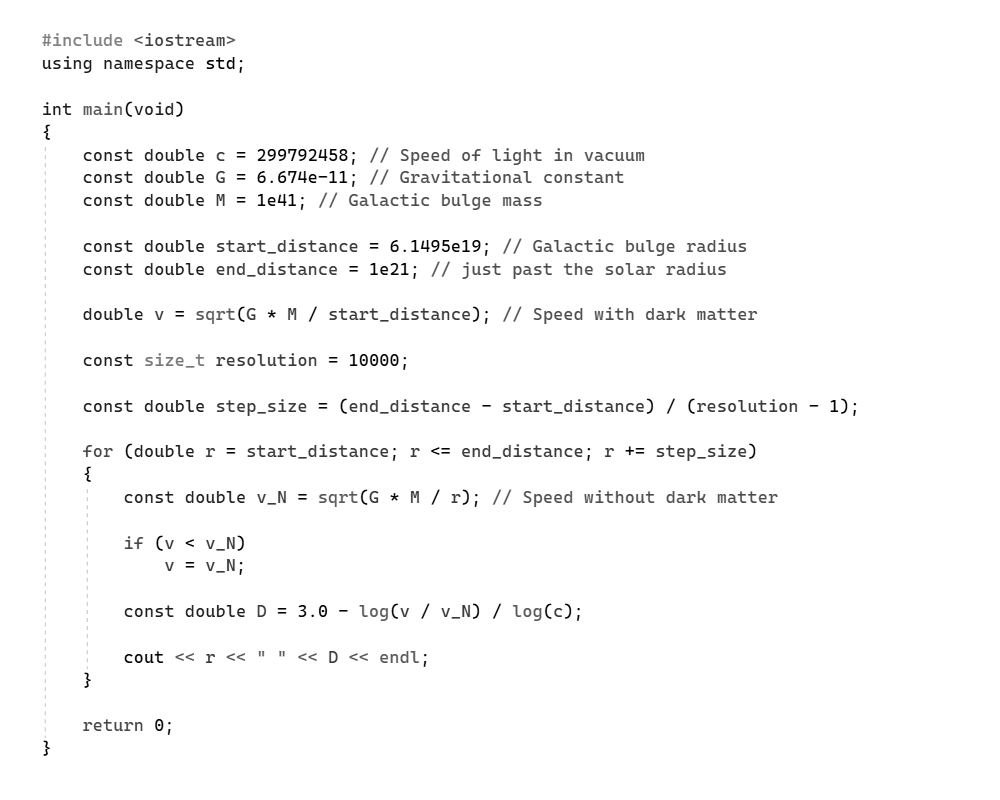
\includegraphics[width = 6 in]{code.png}
  \caption{ C++ code for Galactic orbit. Here $D$ represents dimension.}
\end{figure}


\begin{figure} 
\centering
  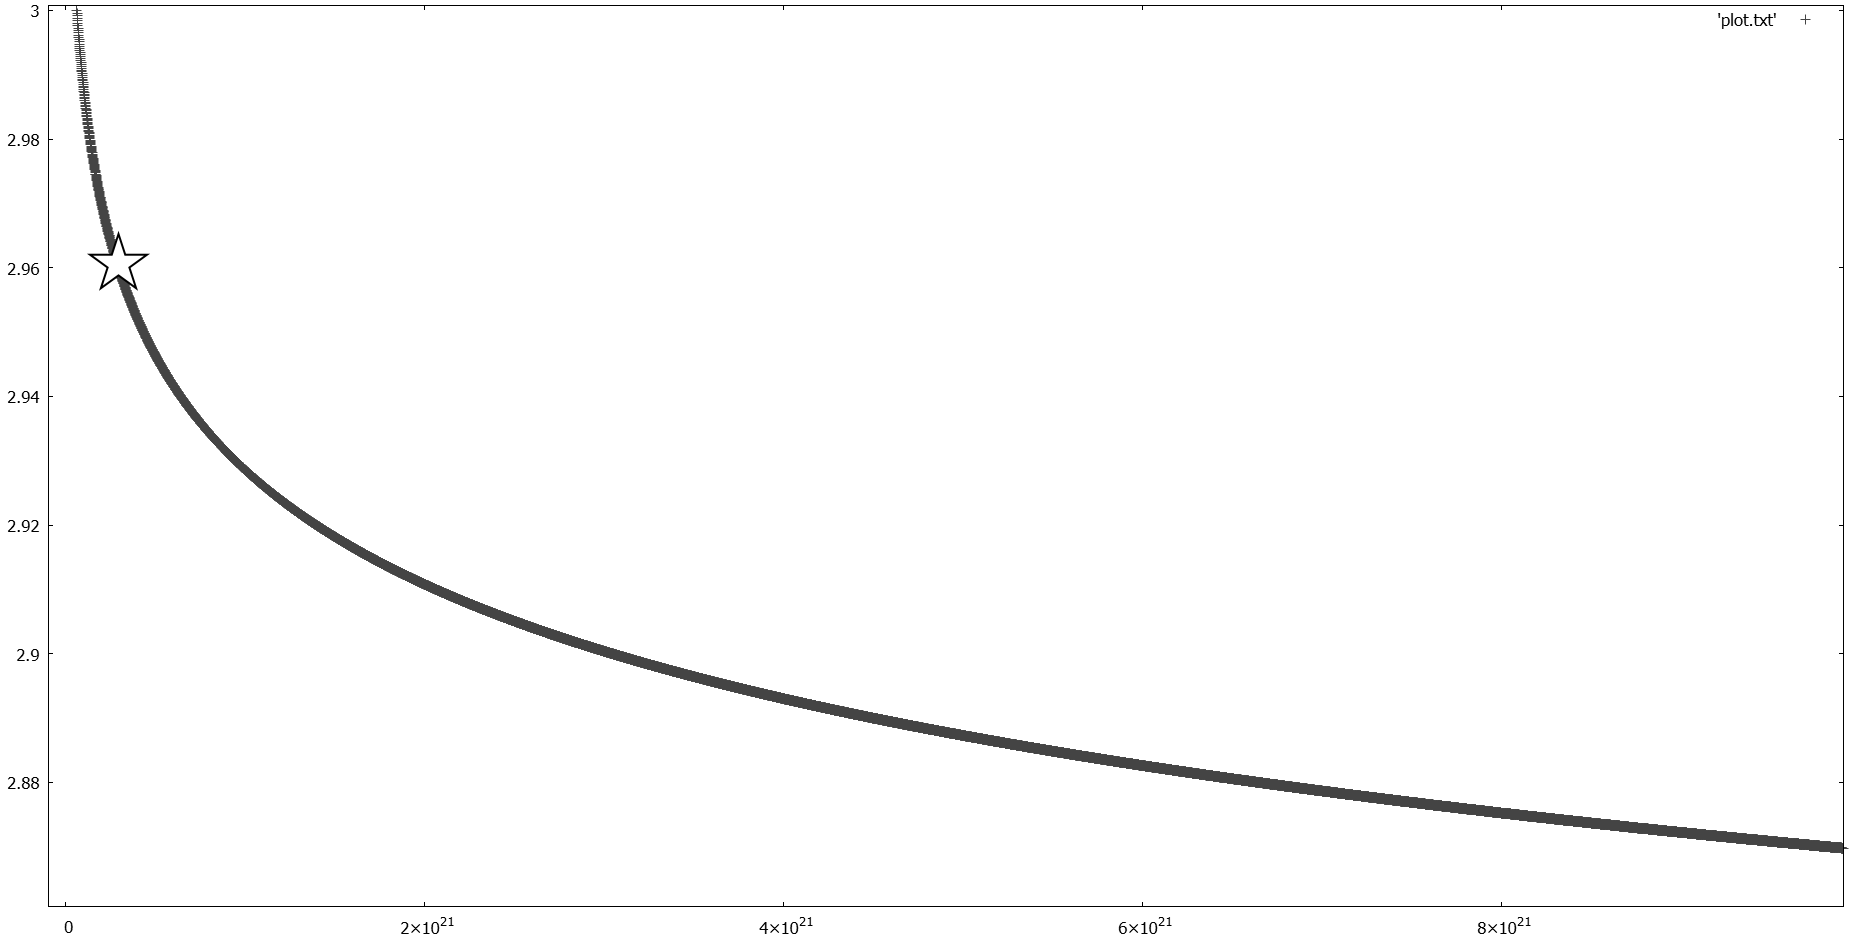
\includegraphics[width = 5 in]{dimension_graph.png}
  \caption{ Here the $x$ axis is the distance from the Galactic centre $r$, and the $y$ axis is dimension $D$.}
\end{figure}




\end{document}









